\documentclass[10pt,a4paper]{article}
\usepackage{nips15submit_e}
\usepackage{amsmath}
\usepackage{mathtools}
\usepackage{amsfonts}
\usepackage{amssymb}
\usepackage{graphicx}
\usepackage{float}
\usepackage{hyperref}
%\usepackage[
%backend=bibtex,
%sorting=unsrt
%]{biblatex}
%\addbibresource{projectsources.bib}
\usepackage{xcolor}
\usepackage{algorithmicx}
\usepackage{algpseudocode}
\usepackage{setspace}

\usepackage[paperwidth=8.5in,paperheight=11in,centering,hmargin=1in,vmargin=1in]{geometry}
\nipsfinalcopy

%\DeclarePairedDelimiter{\norm}{\lVert}{\rVert}
\usepackage{physics}
\newcommand{\prox}{\mathrm{prox}}
\newcommand{\R}{\mathbb{R}}
\newcommand{\C}{\mathbb{C}}
\newcommand{\Tau}{\mathcal{T}}
\newcommand{\AMz}{\underset{z}{arg\, min}}

\begin{document}
\title{Image Deblurring and Denoising for Various Fidelity Terms and Regularizers}
\author{
Kelsey Maass, ~Samuel Rudy, ~Kevin Mueller, ~and Riley Molloy\\
University of Washington\\
}

\maketitle

\begin{center}
\begin{minipage}{0.8\textwidth}
\begin{center}
\textbf{Abstract}
\end{center}
weeee worm weeee worm weeee worm weeee worm weeee worm weeee worm weeee worm weeee worm weeee worm weeee worm weeee worm weeee worm weeee worm weeee worm weeee worm weeee worm weeee worm weeee worm weeee worm weeee worm weeee worm weeee worm weeee worm weeee worm weeee worm weeee worm weeee worm weeee worm weeee worm weeee worm weeee worm weeee worm weeee worm weeee worm weeee worm weeee worm 
\end{minipage}
\end{center}

% Introduction
\section{Introduction}

Image denoising and deblurring problems can be modeled with the linear system
\begin{equation}
Ax + w = b,
\end{equation}
where $b$ is the observed image, $w$ is some unknown noise, and $x$ is the true image we would like to recover. For a blurred image we let $A$ represent the blurring process, and for noisy images we let $A$ be the identity matrix. For many inverse problem applications the least squares approximation, 
\begin{equation}
\hat{x}_{LS} = \arg\min_x \| Ax - b \|_2^2 ,
\end{equation}
gives a reasonable solution. Unfortunately, this approach doesn't provide any new information for the denoising problem, and for image deblurring problems $A$ is often ill-conditioned, so the solution is contaminated by round-off error and amplified noise. To illustrate this, we consider the pepper image below. If we blur the image and compute the naive solution $x = A^{-1}b$, the result is obscured by round-off error in the form of ringing artifacts. The result is even worse when we add noise.

\begin{figure}[H]
\centering
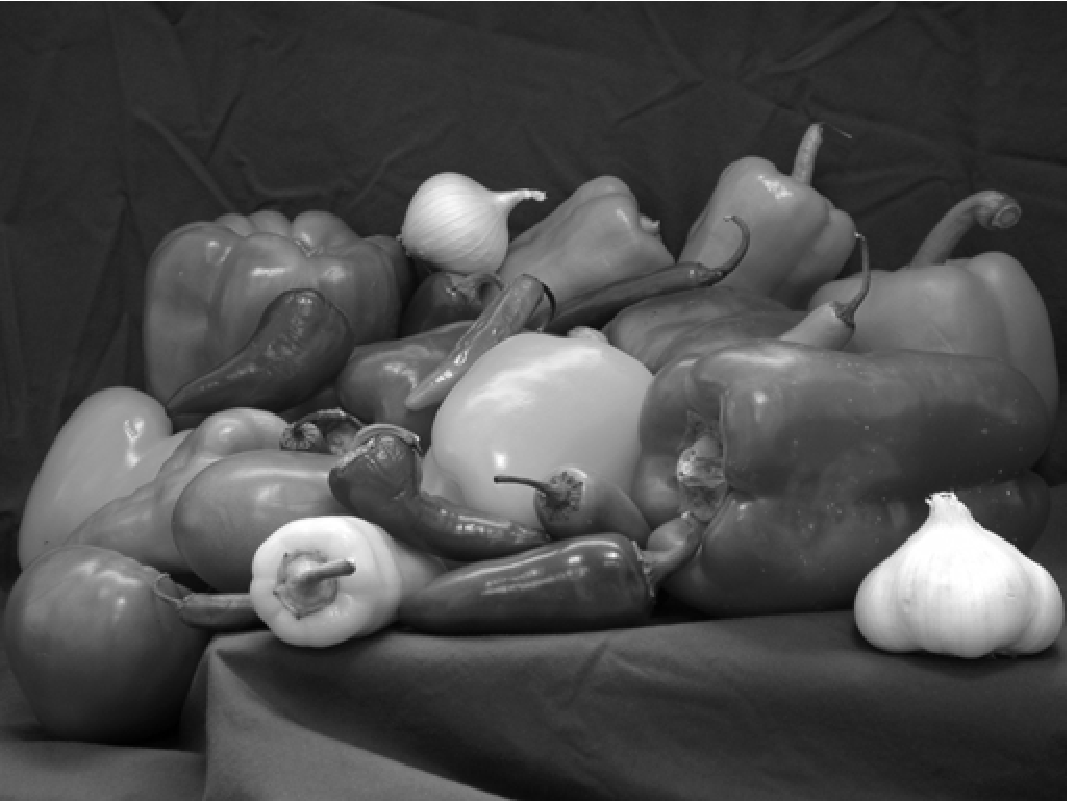
\includegraphics[width=2in]{../figures/fig1}
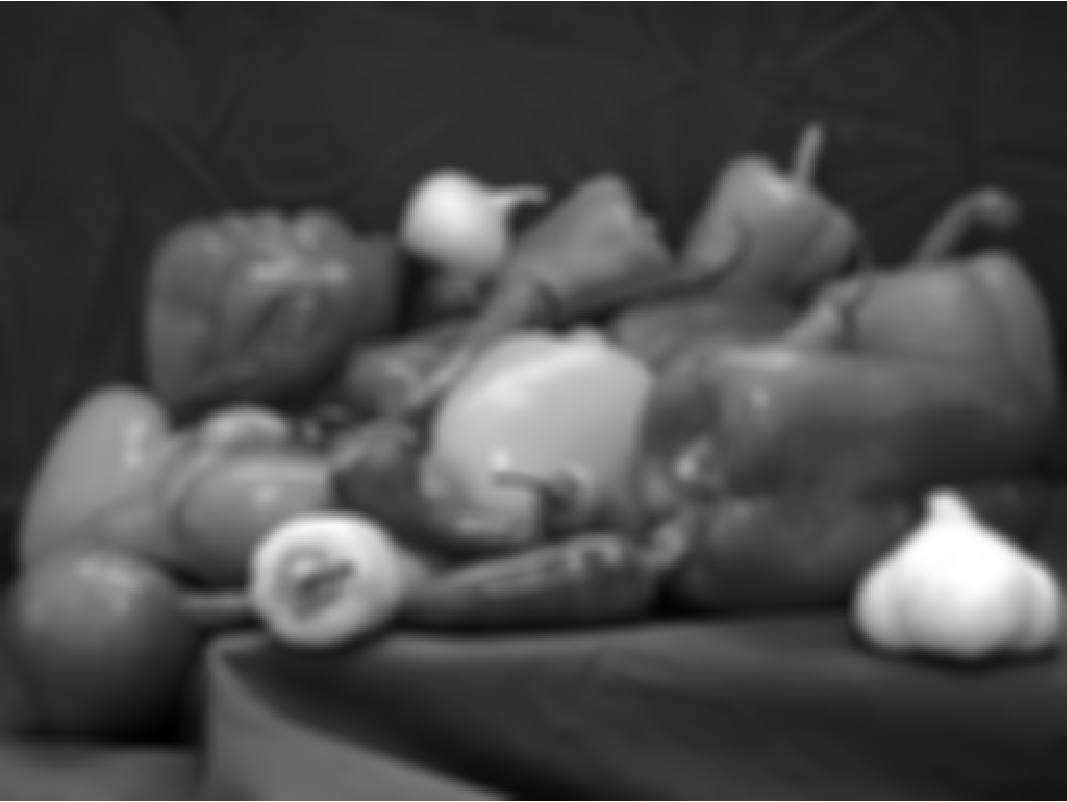
\includegraphics[width=2in]{../figures/fig2}
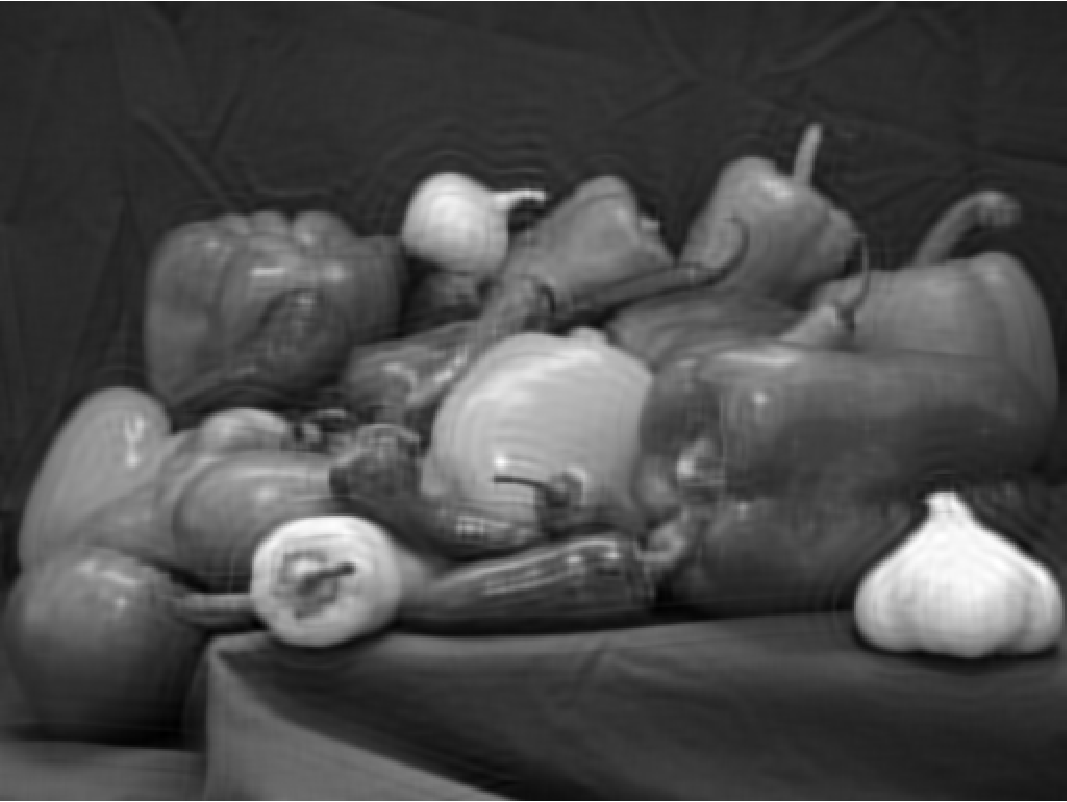
\includegraphics[width=2in]{../figures/fig3} \\[1ex]
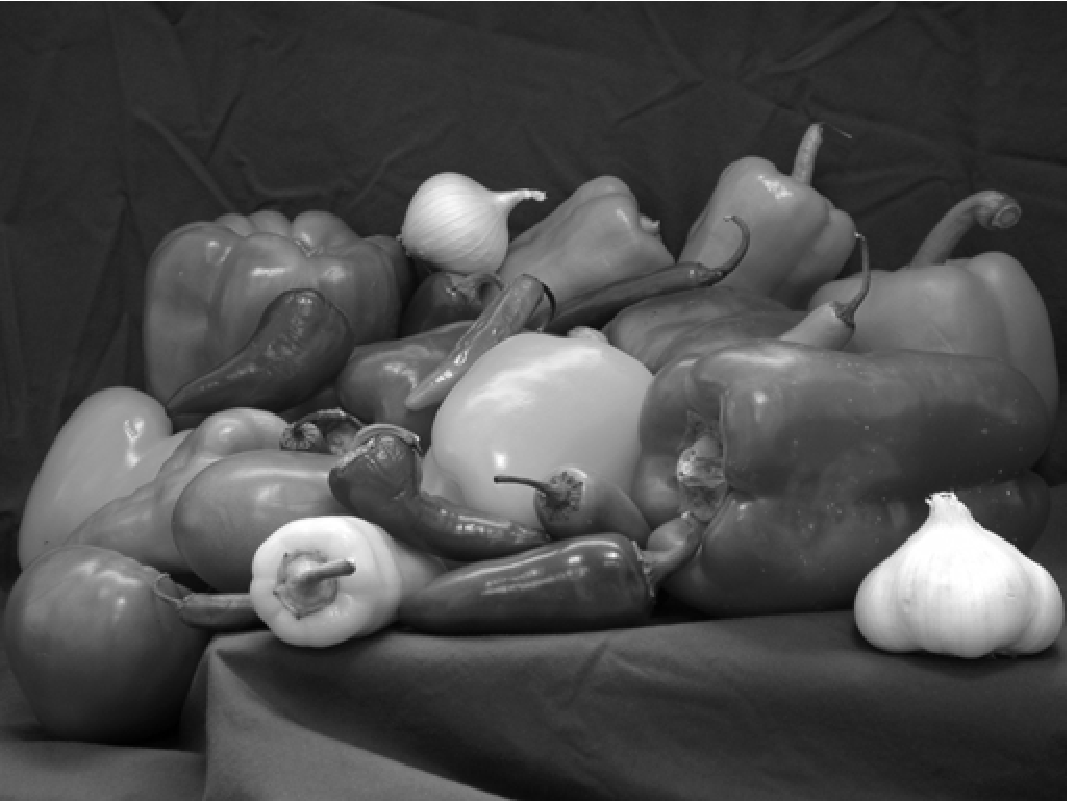
\includegraphics[width=2in]{../figures/fig1}
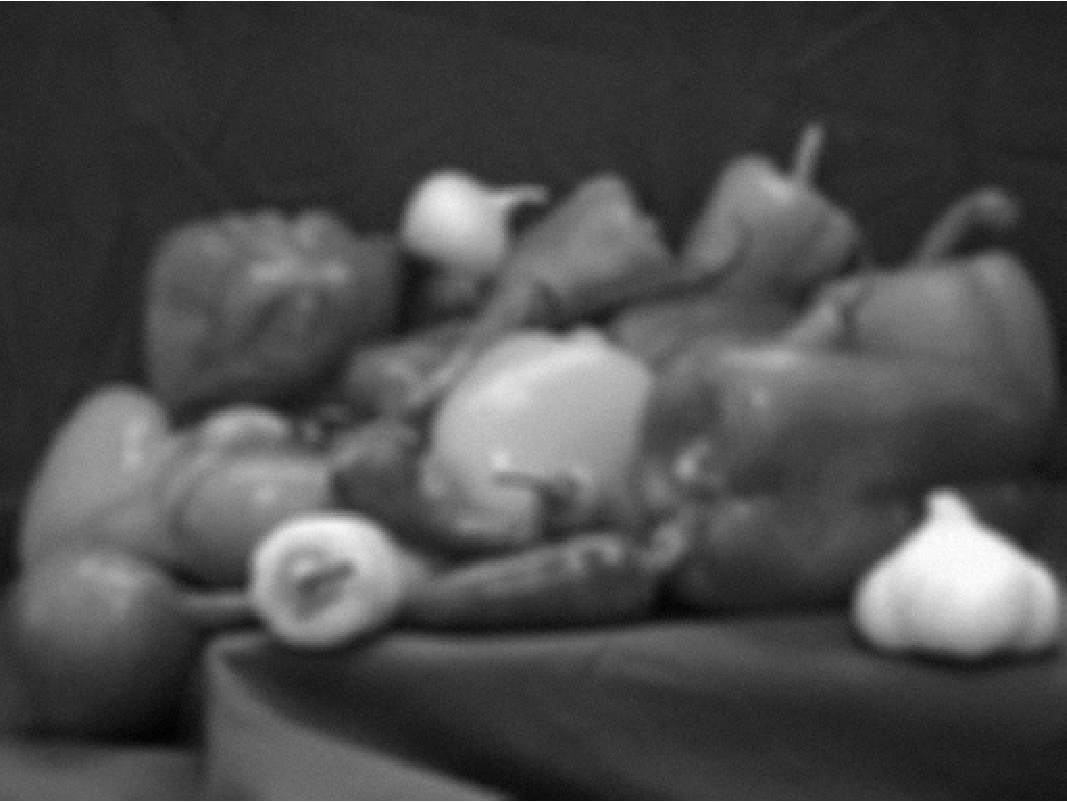
\includegraphics[width=2in]{../figures/fig4}
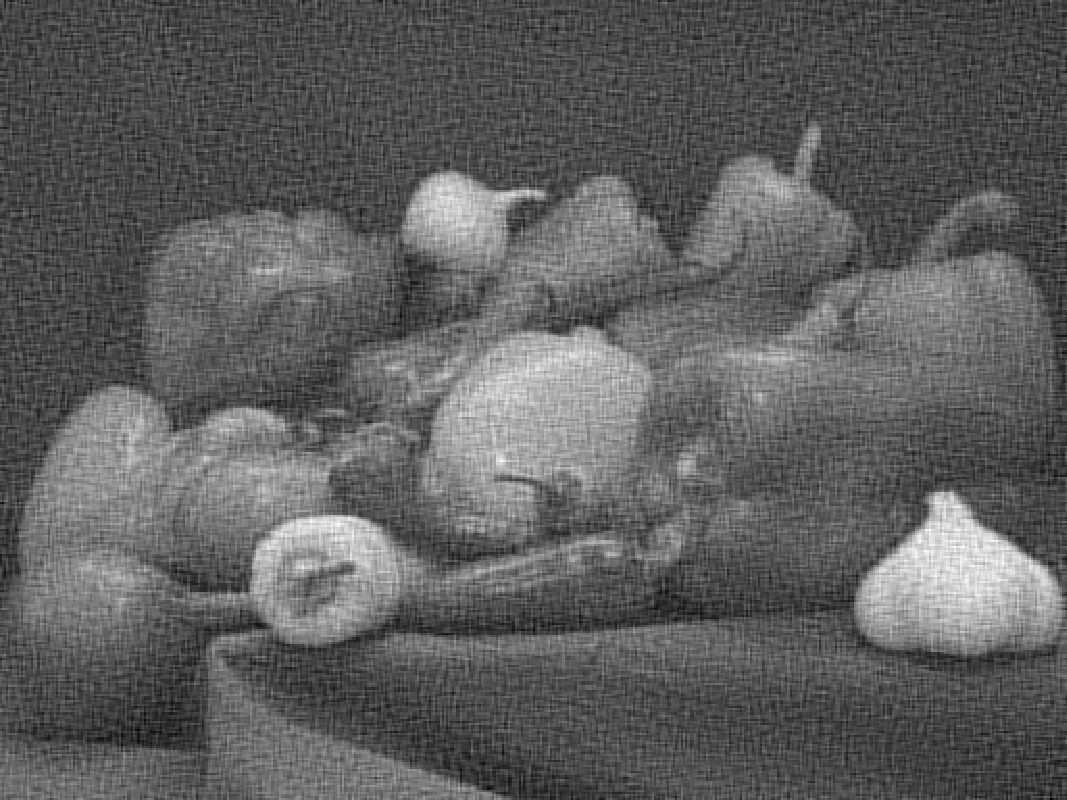
\includegraphics[width=2in]{../figures/fig5}
\caption{\small In the top row we observe the naive solution applied to a blurred image, including the true image $x$ (left), the blurred image $b$ (middle), and the recovered image $A^{-1}b$. On the bottom row, we see the effects of adding noise illustrated by the true image $x$ (left), the blurred and noisy image $b-w$ (middle), and the recovered image $A^{-1}(b-w)$.}
\end{figure}

In order to stabilize the solution, a variety of regularizers can be used which exploit features of the true image such as smoothness or sparsity in a wavelet domain. This results in the problem formulation
\begin{equation}
\hat{x} = \arg\min_{x} \| Ax - b \|_2^2 + \lambda R(x),
\end{equation}
where the parameter $\lambda > 0$ is chosen to balance the tradeoff between fidelity to the model and the assumed feature. In this paper we compare two choices for the regularization term, 
\begin{align}
&\text{Total variation regularization:} &\hat{x}_{TV} = \arg\min_x \| Ax - b \|_2^2 + 2\lambda \| x \|_{TV} , \\
&\text{and } \ell_1 \text{ regularization:} &\hat{x}_{\ell_1} = \arg\min_x \| Ax - b \|_2^2 + \lambda \| Wx \|_1  ,
\end{align}

which are explored by Beck and Teboulle in \cite{TV} and \cite{FISTA} respectively.

It is also known that the quadratic penalty is extremely sensitive to outliers. While this does not pose problems for images with Gaussian noise, which may result from atmospheric turbulence, it becomes an issues for images with noise from heavier tailed distributions, such as the Student's t-distribution, which could result from a dirty camera lens. Therefore we also consider different choices for the fidelity term which are more robust to outliers than the quadratic penalty, including the Huber norm
\begin{equation} \label{huber}
h_{\gamma}(x) = \min_y \frac{1}{2} \| x - y \|_2^2 + \gamma \| y \|_1,
\end{equation}
and the function
\begin{equation} \label{log_cosh}
g_{\gamma}(x) = \frac{1}{\gamma} \sum_i \log\left(\cosh\left(\gamma x_i\right)\right).
\end{equation}

\begin{center}
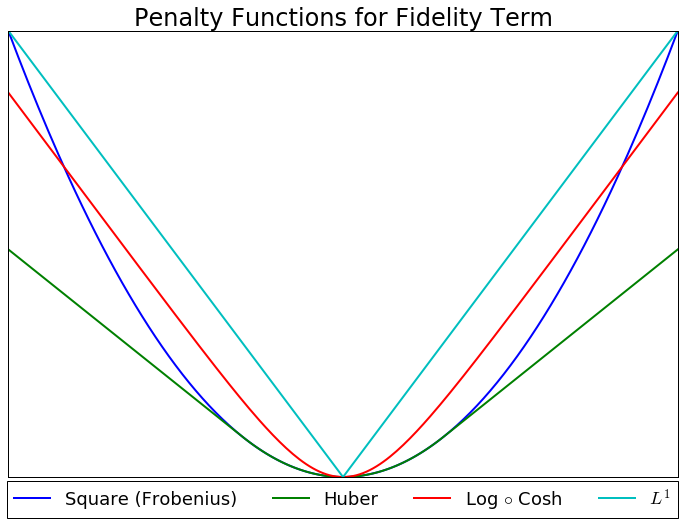
\includegraphics[width=0.8\textwidth]{../figures/penalty_functions.png} 
\end{center}

% Problem Formulation
\section{Problem Formulation}
The general approach of to an image deblurring or denoising problem is the minimization of a loss function of the form \cite{DeblurBook}
\begin{equation} \label{general}
 \min_x f(\mathcal{A}(x) -b) + g(x),
\end{equation}
where $\mathcal{A}(x)$ is a convolution of the desired image $x$ with a gaussian kernel creating a blur,  $f : \R^{m \times n} \rightarrow [0, \infty)$ represents some continuous measure of distance between the corrupt image $b$ and the desired image $x$, and $g:\R^{m \times n} \rightarrow [0,\infty)$ is some regularization on the allowed amount of noise in $x$. The term $f(\mathcal{A}(x)-b)$ is referred to as the \emph{fidelity term}, and the term $g(x)$ is referred to as the \emph{regularization}. We can represent the blurring convolution $\mathcal{A}(\cdot): \R^{m \times n} \rightarrow \R^{m \times n}$ by left matrix multplication with some matrix $A$, so we do so for convenience from here forward. In addition, since we require some pixel value $x_{ij} \in [0,1]$, we can add an additional term to the loss function as
\begin{equation} \label{loss}
 L_b(x) = f(Ax-b) + g(x) + \delta(x | [0,1] ),
\end{equation}
where $\delta(x | [0,1])$ is an indiciator function for the unit interval. 

A simple way to solve for the real image $x$ give $g(x) = 0$ is to apply the gradient descent algorithm,

\begin{equation}
x_k = x_{k-1} - t_k \nabla f(x_{k-1}),
\end{equation}

for suitable stepsize $t_k > 0$. When $g$ is nontrivial and nonsmooth (the usual case), we can rewrite this as a proximal mapping,

\begin{equation}
\prox_g(x_{k-1} - \nabla f(x_{k-1})) = \min_x \left( \frac{1}{2}||x-x_{k-1} - \nabla f(x_{k-1})||_2^2  + \lambda g(x)\right)
\end{equation}

The advantage of this form is that many nonsmooth regularizers have a close formed solution for their $\prox$.

% 1-Norm Wavelet Regularization
\subsection{Wavelet Regularization}

The wavelet regularization deblurring model, as seen in \cite{FISTA}, can be formulated in the form of \eqref{general} as 
\begin{equation} \label{wavelet_orig}
\min_{x} \norm{ Ax - b }_F^2 + \lambda \norm{Wx}_1 ,
\end{equation}
where $\norm{\cdot}_F$ is the Frobenius norm, $\lambda>0$ is a regularization parameter, and $W$ corresponds to a wavelet trasform of a given wavelet type. The primary motivation for this approach is that most images have a sparse representation in the wavelet domain that can be easily exploited by $\ell_1$ regularization. 

Our approach considers a more general problem
\begin{equation} \label{wavelet}
\min_{x} f(Ax - b ) + \lambda \norm{Wx}_1,
\end{equation}
where $f: \R^{m \times n} \rightarrow [0,\infty)$ is some Lipschitz differentiable functional which gives a measurement of the size of the fidelity term. We specifically work with the cases 
\begin{equation} \label{fidelities}
f(x) = \begin{cases}
\norm{x}_F^2 \\
h_\gamma(x) \\
g_\gamma(x),
\end{cases}
\end{equation}
where $h_\gamma$ and $g_\gamma$ are as in \eqref{huber} and \eqref{log_cosh} respectively. 

% TV Regularization
\subsection{Total Variation Regularization}
The usual Total-Variation deblurring model, as seen in \cite{TV} can be formulated in the form of \eqref{general} as 
\begin{equation} \label{tv_orig}
\min_{x} \norm{ Ax - b }_F^2 + 2 \lambda \mathrm{TV}(x),
\end{equation}
where $\norm{\cdot}$ is taken as either a Frobenius norm or a 2-norm, depending on applications,  $\lambda>0$ is a regularization parameter, and $\mathrm{TV}(x)$ is the Total-Variation semi-norm. Two similar choices exist for the TV-norm: the so-called isotropic type, and the $l_1$ type.  In this work, we work exclusively with the $l_1$-based TV-norm, defined as 
$$ TV_{l_1}(x) = \sum_{i=1}^{m-1} \sum_{j=1}^{n-1} \left( \abs{x_{i,j}  - x_{i+1,j} } + \abs{ x_{i,j} - x_{i,j+1}  } \right) + \sum_{i=1}^{m-1} \abs{ x_{i,n} - x_{i+1,n} } + \sum_{j=1}^{n-1} \abs{ x_{m,j} - x_{m,j+1 } },$$
 for $x \in \R^{m \times n},$ and where the reflexive boundary conditions
\begin{align*}
x_{m+1,j} - x_{m,j} &= 0, \textrm{ for all }j \\
 x_{i,n+1} - x_{i,n} &= 0, \textrm{ for all }i
\end{align*}
are assumed.  However, it is a very simple adjustment to use the isotropic definition of total variation and all of the same methods still apply. Our approach considers a more general problem
\begin{equation} \label{tv_ours}
\min_{x} f(Ax - b ) + \lambda \mathrm{TV}_{l_1}(x) + \delta(x | [0,1]),
\end{equation}
where $f: \R^{m \times n} \rightarrow [0,\infty)$ is any functional with Lipschitz continuous gradient which gives a measurement of the size of the fidelity term.  In our work, we used the standard Frobenius norm, the Huber penalty, and $\gamma^{-1}\log( \cosh (\gamma \cdot ))$ evaluated element wise in the matrix and summed.\\

Optimization of the objective function was based on the proximal gradient algorithm and expoited the idea of momentum used in FISTA as well as an extra function evaluation at each iteration in order to ensure a non-increasing objective function.  The proximal gradient step is given as follows,

\begin{align*}
x^{k+1} &= \prox_{\alpha^{-1}(\lambda \|\cdot \|_{TV} + \delta_{[0,1]})} (\underbrace{x^k - \alpha^{-1} A^T\nabla f (Ax^k - b)}_{u^k}) \\
&= \AMz \left( \|u^k - z\|_F^2 + \alpha^{-1}\lambda TV(z) + \delta(z | [0,1]) \right) \\
&= P_{[0,1]}  \left( \AMz \left( \|u^k - z\|_F^2 + \alpha^{-1}\lambda TV(z) \right) \right)
\end{align*}

Here the learning rate $\alpha$ is taken to be no larger than than the multiplicative inverse of the Lipschitz constant of $\nabla f$.  Note that in order to evaluate this expression we must solve a denoising problem with input $u^k = x^k - \alpha^{-1} A^T\nabla f (Ax^k - b)$.  Of particular note is that regardless of the original fidelity term we have a Frobenius norm fidelity term on the new denoising problem.  This allows for the easy manipulation of the original fidelity function, so long as it is convex and has Lipschitz gradient.

The resulting denoising problem with Frobenius norm fidelity function may be solved rapidly using the method developed in \cite{TV}.  The $TV$ function is shown to have a dual representation as a trace and the relationship between trace and Frobenius norm is heavily exploited to develop a dual formulation of the denoising problem.  We present their method here, starting with a few new definitions which will be necessary.
\begin{align*}
\mathcal{P} &= \{ (p,q) \in \R^{(m-1) \times n} \times \R^{ m \times (n-1) } :  \abs{p_{i,j} } \le 1, \abs{p_{ i,j } } \le 1 \} \\
 \mathcal{L} : \R^{(m-1) \times n} \times& \R^{ m \times (n-1) } \rightarrow \R^{m \times n}  \text{ such that } \mathcal{L}(p,q)_{i,j} = p_{i,j} + q_{i,j} - p_{ i-1,j } - q_{ i,j-1 }\\ &\hspace{3 cm} \text{ for } i = 1,\dots,m,\,j = 1,\dots,n \text{ \& }  p_{0,j} = p_{m,j} = q_{i,0} = q_{i,n} = 0\\
\end{align*}


% Algorithms
\section{Algorithms}

\begin{minipage}{0.48\textwidth}
\textbf{MFISTA$(b,f, \lambda)$}
\begin{algorithmic}
\State $y^1 = x^0 = b; \, t^1 = 1$
\State $\alpha \geq Lip(\nabla f)$
\For {$k = 1:N$}
	\State $u^k = y^k - \frac{A^T\nabla f (A y^k - b)}{\alpha}$
	\State $z^k = FGP(u^k, \frac{\lambda}{2 \alpha})$
	\State $x^k = \underset{x \in \{x^{k-1},z^k\}}{\text{argmin}} \,L_b(x)$
	\State $t^{k+1} = \frac{1 + \sqrt{1 + 4{t^k}^2}}{2}$ 
	\State $y^{k+1} = x^k + \frac{t^k}{t^{k+1}}(z^k - x^k)$ 
	\State \hspace{10 mm}$+ \frac{t^{k-1}}{t^{k+1}}(z^k - x^k) $
\EndFor\\
\Return $x^N$
\end{algorithmic}
\end{minipage}
\begin{minipage}{0.48\textwidth}

\textbf{FGP$(b, \lambda)$}
\begin{algorithmic}
\State $(r_{ij}^1, s_{ij}^1) = (p_{ij}^0, q_{ij}^0) = 0; \, t^1 = 1$
\For {$k = 1:N$}
	\State $(p^k,q^k) = P_\mathcal{P} \left( (r^k,s^k) - \frac{\mathcal{L}^TP_{[0,1]} (b - \lambda \mathcal{L}(r^k,s^k))}{8\lambda} \right)$
	\State $t^{k+1} = \frac{1 + \sqrt{1 + 4{t^k}^2}}{2}$ 
	\State $(r^k,s^k) = (p^k,q^k) + \frac{t^k-1}{t^{k+1}}(p^k-p^{k-1}, q^k-q^{k-1})$ 
\EndFor \\
\Return $P_{[0,1]} (b - \lambda \mathcal{L}(p^N,q^N))$
\end{algorithmic}

\end{minipage}

\subsection{Wavelet Regularization}

\subsection{Total Variation Regularization}

% Examples
\section{Examples}

\subsection{Wavelet Regularization}


\begin{figure}[H]
\begin{center}
\rotatebox{90}{\hspace{1cm} Original Image \hspace{3cm} Frobenius Loss}
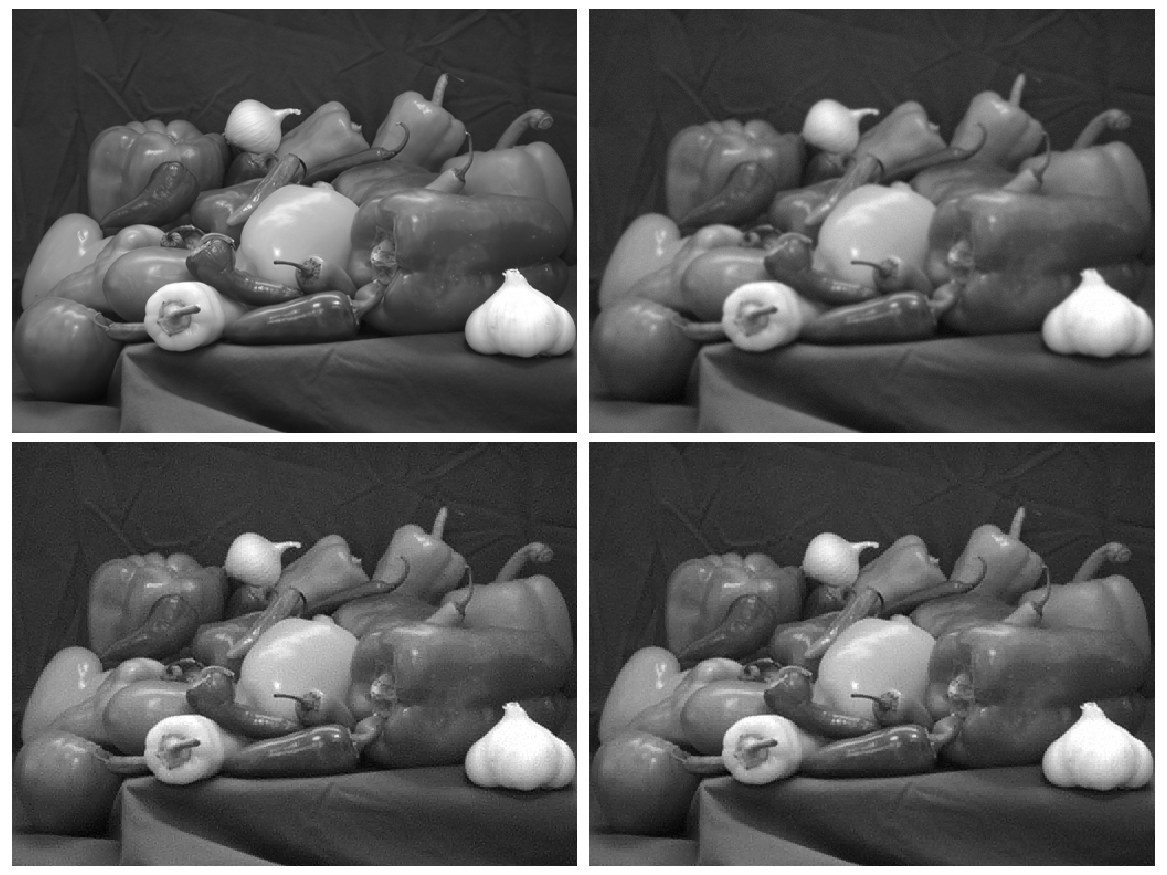
\includegraphics[width = 0.75\textwidth]{../figures/waveletGaussH.pdf} 
\rotatebox{270}{\hspace{-9cm} Blurred and Noisy \hspace{2.6cm} Huber Loss}
\end{center}
\caption{$\ell_1$ Wavelet algorithm performed on an image with Gaussian noise (magnitude $1 \times 10^{-3}$) for the two different fidelity terms of Frobenius and Huber loss. This method used the Haar wavelet for deblurring.}
\label{waveletH_gauss}
\end{figure}

\begin{figure}[H]
\begin{center}
\rotatebox{90}{\hspace{1cm} Original Image \hspace{3cm} Frobenius Loss}
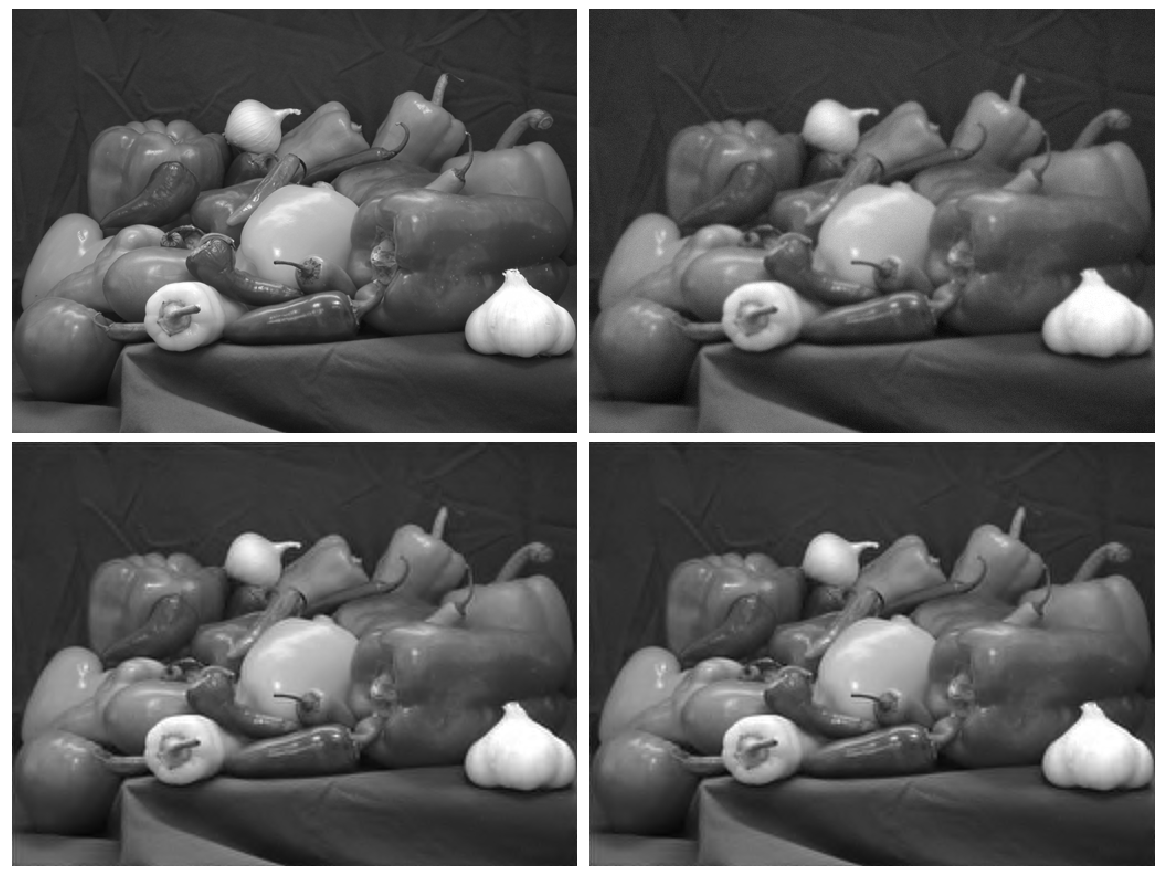
\includegraphics[width = 0.75\textwidth]{../figures/waveletGaussD.pdf} 
\rotatebox{270}{\hspace{-9cm} Blurred and Noisy \hspace{2.6cm} Huber Loss}
\end{center}
\caption{$\ell_1$ Wavelet algorithm performed on an image with Gaussian noise (magnitude $1 \times 10^{-3}$) for the two different fidelity terms of Frobenius and Huber loss. This method used the Daubechies wavelet for deblurring.}
\label{waveletD_gauss}
\end{figure}

\begin{figure}[H]
\begin{center}
\rotatebox{90}{\hspace{1cm} Original Image \hspace{3cm} Frobenius Loss}
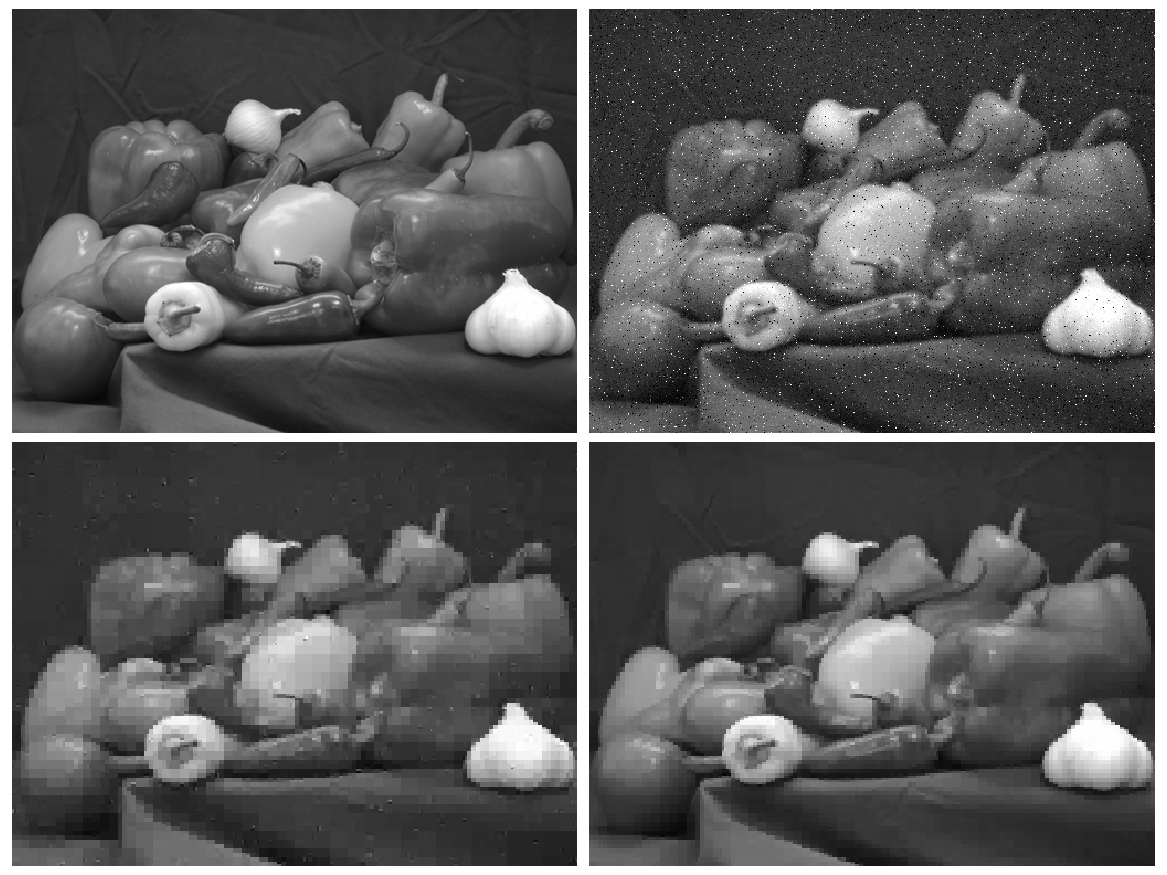
\includegraphics[width = 0.75\textwidth]{../figures/waveletStudentH.pdf} 
\rotatebox{270}{\hspace{-9cm} Blurred and Noisy \hspace{2.6cm} Huber Loss}
\end{center}
\caption{$\ell_1$ Wavelet algorithm performed on an image with Student's t noise (magnitude $1 \times 10^{-4}$) for the two different fidelity terms of Frobenius and Huber loss. This method used the Haar wavelet for deblurring.}
\label{waveletH_student}
\end{figure}

\begin{figure}[H]
\begin{center}
\rotatebox{90}{\hspace{1cm} Original Image \hspace{3cm} Frobenius Loss}
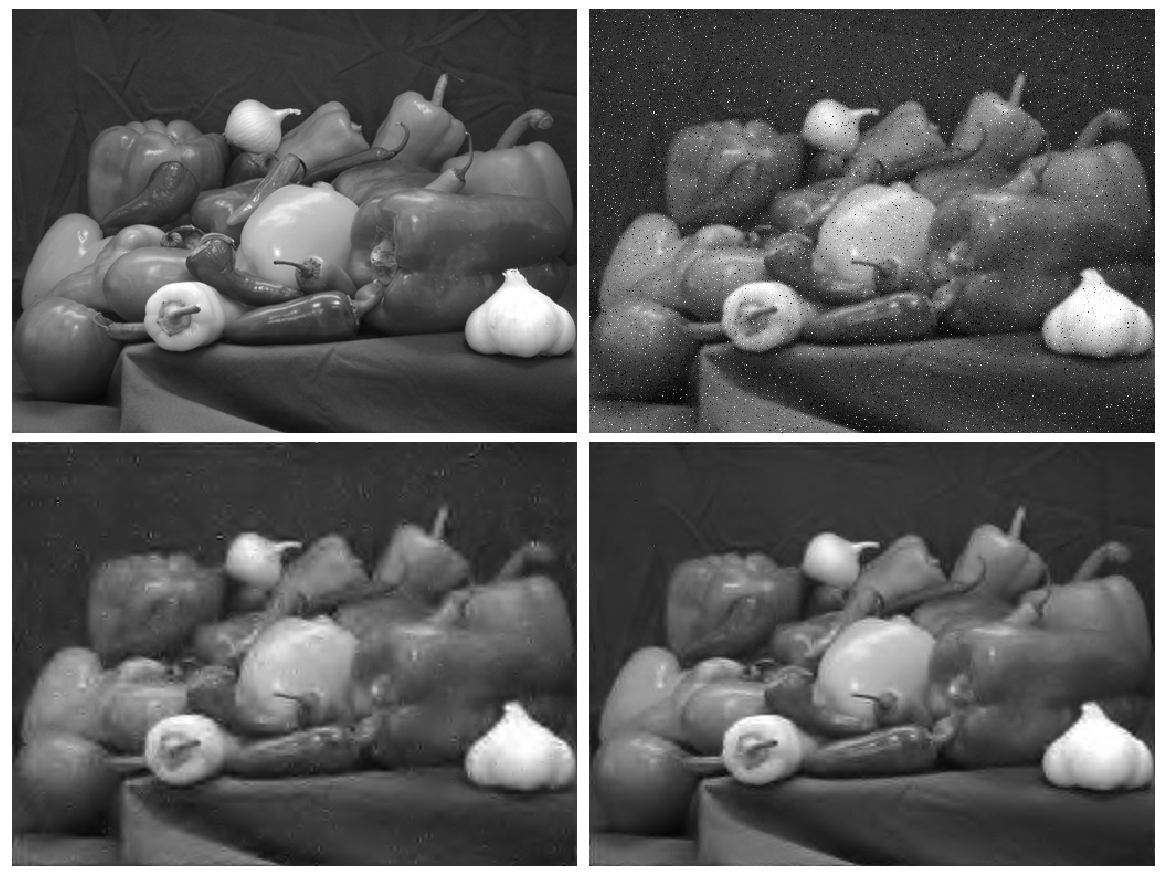
\includegraphics[width = 0.75\textwidth]{../figures/waveletStudentD.pdf} 
\rotatebox{270}{\hspace{-9cm} Blurred and Noisy \hspace{2.6cm} Huber Loss}
\end{center}
\caption{$\ell_1$ Wavelet algorithm performed on an image with Student's t noise (magnitude $1 \times 10^{-4}$) for the two different fidelity terms of Frobenius and Huber loss. This method used the Daubechies wavelet for deblurring.}
\label{waveletD_student}
\end{figure}

\subsection{Total Variation Regularization}

We demonstrate some results of denoising and deblurring with the Total Variation regularization on real images. As previously shown, each image was given a small amount of either Gaussian or Student's t noise and blurred. Two different fidelity functions were used: the squared Frobenius norm, and the Huber norm. Figure \ref{tv_gauss} demonstrates the results using Gaussian noise, and Figure \ref{tv_student} demonstrates the results using Student's t noise with one degree of freedom. For the Gaussian noise, we set $\lambda = .001$, and $\gamma = .02$ (see TV-regularization in Problem Formulation). For Student's t noise, we set $\lambda = .002$, and $\gamma = .02$.

\begin{figure}[H]
\begin{center}
\rotatebox{90}{\hspace{1cm} Original Image \hspace{3cm} Frobenius Loss}
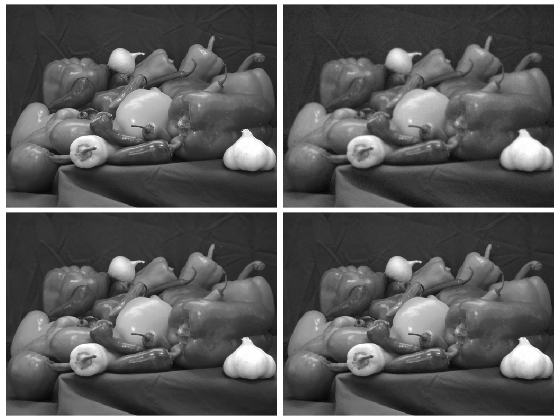
\includegraphics[width = 0.75\textwidth]{../figures/gaussian_peppers.png} 
\rotatebox{270}{\hspace{-9cm} Blurred and Noisy \hspace{2.6cm} Huber Loss}
\end{center}
\caption{Total Variation algorithm performed on an image with Gaussian noise (magnitude $1 \times 10^{-3}$) for the two different fidelity terms of Frobenius and Huber loss.}
\label{tv_gauss}
\end{figure}

\begin{figure}[H]
\begin{center}
\rotatebox{90}{\hspace{1cm} Original Image \hspace{3cm} Frobenius Loss}
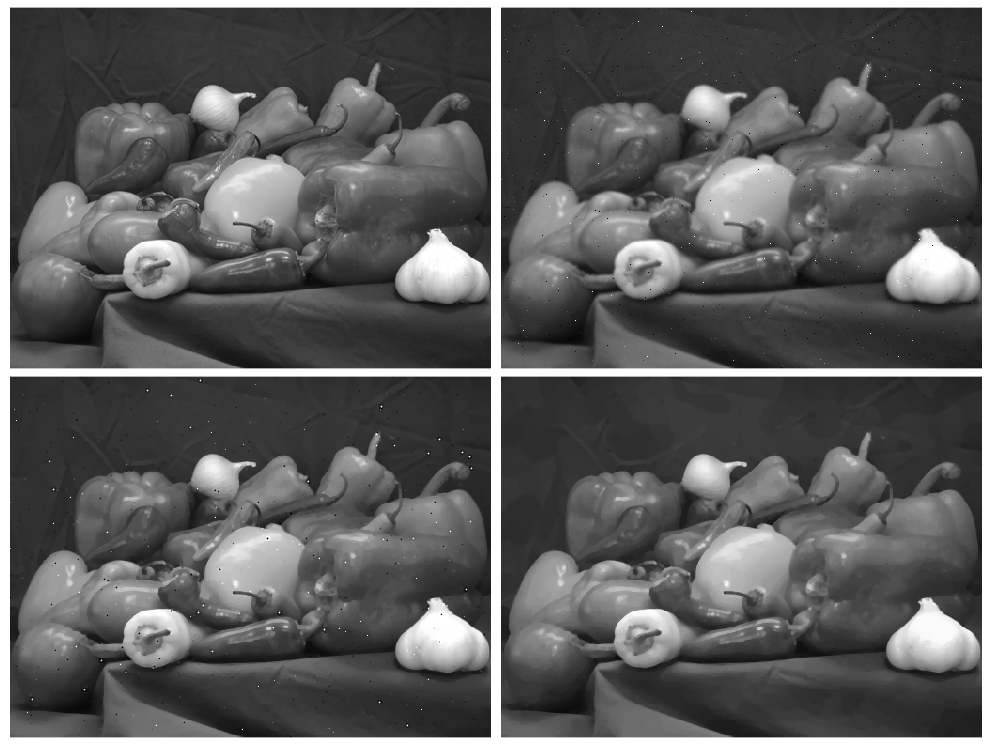
\includegraphics[width = 0.75\textwidth]{../figures/student-t_peppers.png} 
\rotatebox{270}{\hspace{-9cm} Blurred and Noisy \hspace{2.6cm} Huber Loss}
\end{center}
\caption{Total Variation algorithm performed on an image with Student's t noise (magnitude $1 \times 10^{-4}$) for the two different fidelity terms of Frobenius and Huber loss.}
\label{tv_student}
\end{figure}


\begin{figure}[H]
	
	\begin{center}
		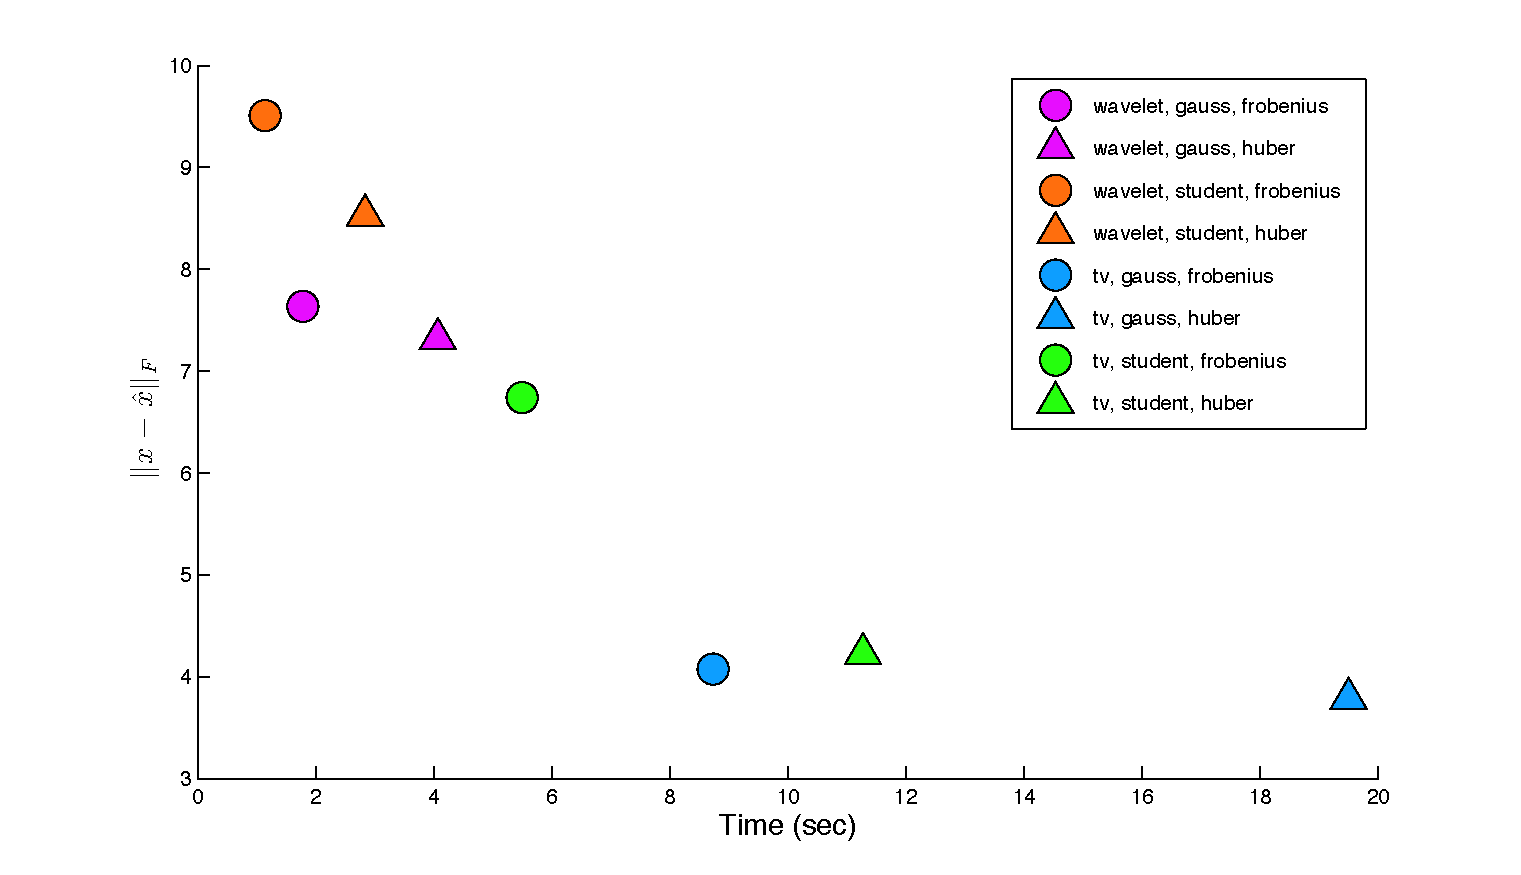
\includegraphics[width=0.8\textwidth]{../figures/comparePlot2.pdf}
		\caption{Timing information and the Frobenius norm error between the true and observed image until the relative change in the objective function is less than $.001$. }
		\label{comp_methods}
	\end{center}
\end{figure}


Figure \ref{comp_methods} shows a rough comparison of our methods by displaying the time complexity and Frobenius error for different fidelity functions, regularization techniques and noise-types. It is clear that TV regularization outperformed wavelet regularization at the price of additional computational complexity. This is not surprising due to TV's extra requirement of solving an inner optimization problem for denoising the image. It can also be seen that student noise generally required less time than Gaussian noise but at the expense of higher error. Finally, applying the Huber for student noise improved results drastically for a slight increase in computation time.  

% Discussion
\section{Discussion and Conclusions}

In conclusion, we present a survey of regularization and fidelity functions for the image denoising/deblurring problem. In particular, we compare regularization of the 1-norm in the wavelet domain to TV regularization. Furthermore we explore the affect of using the Huber as a fidelity function and potential improvements it can have when applied to heavy tailed noise. Our results show that TV regularization performs better for high amounts of noise, but the wavelet domain is well suited for smaller amounts of noise due to computational speed improvements. 

In our research we came across many challenges and avenues for future work. It is clear from \ref{lambda_find}, that the correct choice of the regularization parameter is very important for maximizing results. However, the correct value varies for different classes of images. Therefore, there is a high need for finding the correct value for the regularization parameter across images. Additionally, finding an appropriate error metric can be a difficult challenge when quantitatively analyzing performance for the methods shown. The Frobenius norm of the error is the most common metric, but does can do a poor job of correctly evaluating the improvements from denoising and deblurring algorithms due to large structural changes of the images. 





%\printbibliography[title={Sources}]
\bibliographystyle{unsrt}
\bibliography{sources}


\end{document}